\pdfminorversion=4
\documentclass[aspectratio=169]{beamer}
\usepackage{verbatim}
\newenvironment{metaverbatim}{\verbatim}{\endverbatim}
\usepackage{courier}
\usepackage{lmodern}
\usepackage{apacite}
\usepackage[hidelinks]{hyperref}
\usepackage{xcolor}
\xdefinecolor{azulcesafuerte}{HTML}{14387e}
\xdefinecolor{azulcesaclaro}{HTML}{7ab6e0}
\xdefinecolor{azulcesamedio}{HTML}{0A72BC}

\usetheme{Madrid}
%\usecolortheme[named=black]{structure}
%
\setbeamercolor{normal text}{fg=azulcesafuerte}
\setbeamercolor{background canvas}{bg=white}
\setbeamercolor{frametitle}{fg=white, bg=azulcesafuerte}
\setbeamercolor{block title}{bg=azulcesafuerte,fg=azulcesaclaro}
\setbeamercolor{navigation symbols}{}

\setbeamertemplate{background}{\tikz[overlay,remember picture]\node[opacity=0.15]at (current page.center){\includegraphics[width=6.5cm]{}};}
\usepackage{tikz}
\usepackage{kantlipsum}
\setbeamercolor*{title}{fg=white, bg=azulcesafuerte}
\setbeamercolor{titlelike}{parent=structure}

\setbeamercolor*{palette primary}{bg=azulcesafuerte,fg=white}
\setbeamercolor*{palette secondary}{bg=azulcesafuerte,fg=white}
\setbeamercolor*{palette tertiary}{bg=azulcesafuerte,fg=white}

% Change base colour beamer@blendedblue (originally RGB: 0.2,0.2,0.7)
\colorlet{beamer@blendedblue}{azulcesaclaro}
\usepackage[spanish]{babel}
\usepackage{apacite}
\usepackage{marvosym}
\usepackage{subfig}
\usepackage{graphicx}
\usepackage[utf8x]{inputenc}
\usepackage{url}
\usepackage{hyperref}
\usepackage{times}
\usepackage{pxfonts}
\usepackage{fontenc}
%\usepackage[dvipsnames]{xcolor}
\setbeamertemplate{bibliography item}[text]
\title[Fundamentos de Analítica de Datos]{Fundamentos de Analítica de Datos}
\subtitle{(Sesión 4B)}

\author[Prof. Juan C. Correa, Ph.D.]{Prof. Juan C. Correa, Ph.D.}

\institute[]{
Colegio de Estudios Superiores de Administración\\
Bogotá - Colombia\\
% \color{azulcesaclaro}\Email  \href{mailto:juan.correan@cesa.edu.co}{juan.correan@cesa.edu.co}
}
\pgfdeclareimage[height=0.6cm]{OL}{OL}
 \logo{\pgfuseimage{OL}}
 \setbeamertemplate{caption}[numbered]
\date[Bogotá, Agosto, 2021] % (optional)
{}

\subject{}
\begin{document}
\begin{frame}
\titlepage
\end{frame}

% \begin{frame}
% \frametitle{Agenda} 
% \tableofcontents
% \end{frame}

\begin{frame}
\begin{block}{Objetivo de Aprendizaje}
En la Sesión 4A, se ilustró la lógica de la analítica de datos al explicar por qué las limitaciones de Excel conllevan a la necesidad de usar otras herramientas más adecuadas (e.g., Anaconda-Navigator, jupyter Notebook, Python Pandas). Al finalizar este sesión, usted aprenderá a aplicar algunas técnicas sencillas de visualización de datos con otras herramientas profesionales (i.e., Jamovi, RStudio) que le facilitarán su aprendizaje con los lenguajes de programación.
\end{block}
\end{frame}

\section{Insumos Preliminares}
\begin{frame}
\begin{center}
\Huge
\textcolor{azulcesaclaro}{1\\
--------------------------------\\
Insumos Preliminares}
\end{center}
\end{frame}

\begin{frame}
Para esta sesión necesitamos descargar e instalar \href{https://www.jamovi.org/}{\textcolor{blue}{Jamovi}}. También necesitamos descargar e instalar  \href{https://youtu.be/Bg2LzHmPZFY}{\textcolor{blue}{R y Rstudio}}
\begin{figure}
    \centering
    
\includegraphics[width=.65\textwidth]{InstalaR.png}
\end{figure}
\end{frame}

\begin{frame}
Para esta sesión, también necesitaremos descargar la base de datos descrita en el artículo de \citeauthor{Segura2019} \citeyear{Segura2019} disponible \href{https://doi.org/10.1016/j.dib.2019.104007}{\textcolor{blue}{aquí}} y \href{https://data.mendeley.com/datasets/m9z9hw4nsc/1}{\textcolor{blue}{aquí}}. Para comprender el contexto empírico donde se desarrolló esta base de datos, basta con repasar algunos detalles mencionados en el artículo de \citeauthor{Correa2019} \citeyear{Correa2019}. De inmediato se ofrece un resumen.\\
\begin{figure}
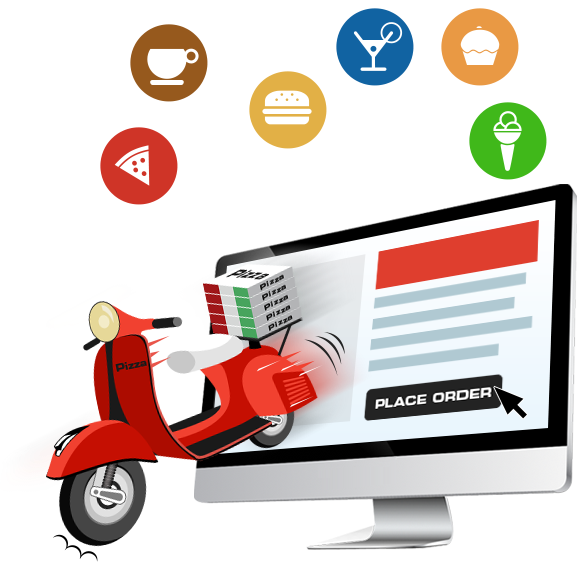
\includegraphics[width=.3\textwidth]{ofos}
\end{figure}
\end{frame}

\begin{frame}
Aplicando técnicas de minería web, se recolectaron los datos de las siguientes variables para un total de 787 restaurantes indexados en la página de domicilios.com, 4296 clientes y 19934 rutas cubiertas en tres horas pico de tráfico sabatino de Bogotá:
\vspace{0.5cm}
\begin{itemize}
    \item Número de Comentarios (indicador de Consumo Colaborativo)
    \item Pedido Mínimo
    \item Costo del domicilio
    \item Tiempo de entrega esperado
    \item Cumplimiento en el tiempo de entrega (según estimados de Google Maps) 
\end{itemize}
\end{frame}

\begin{frame}
\begin{figure}
\centering
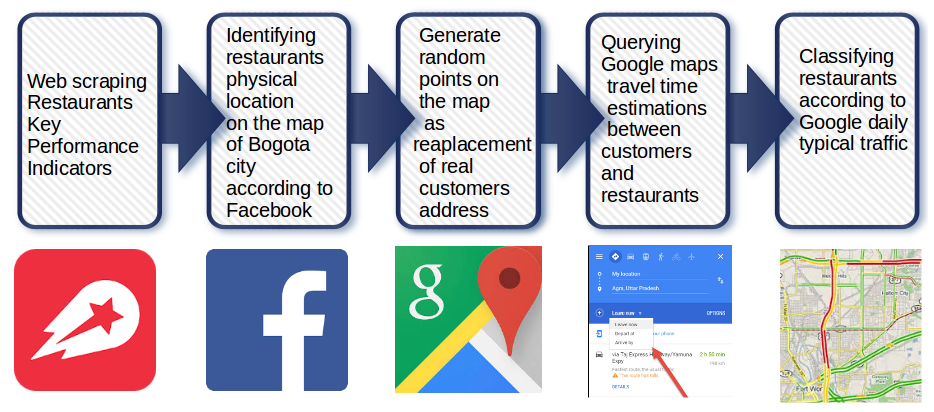
\includegraphics[width=0.9\textwidth]{procedure.png}
\end{figure}
\end{frame}

\begin{frame}
Antes de practicar, necesitamos entender qué es una \textbf{sintaxis}:
\begin{figure}
\centering

\includegraphics[width=0.9\textwidth]{sintaxis.png}
\end{figure}
Una sintaxis es una orden escrita por una persona para que una computadora se encargue de cumplirla. Las sintaxis se escriben en un lenguaje comprensible por la computadora. Las sintaxis usualmente combinan dos elementos: funciones y argumentos. Veamos algunos ejemplos.
\end{frame}

\begin{frame}
Aquí hay dos \textbf{sintaxis}. La de arriba está escrita con lenguaje Python. La de abajo con lenguaje R. 
\begin{figure}
\centering
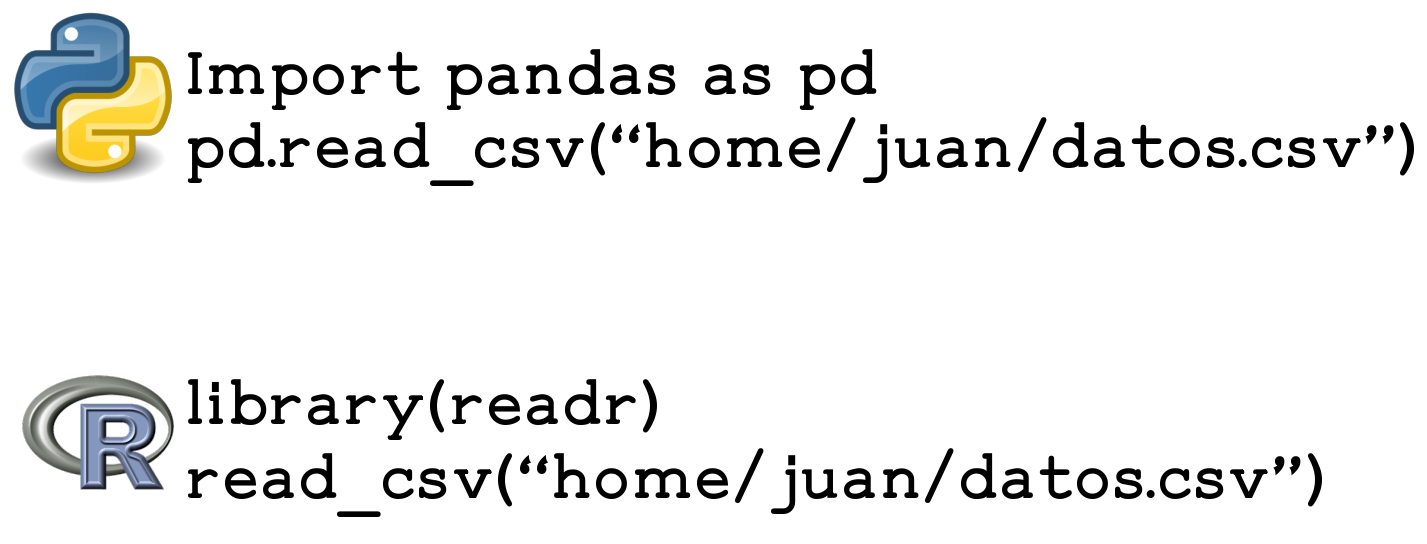
\includegraphics[width=0.8\textwidth]{sintax.png}
\end{figure}
La función está por fuera del paréntesis y el argumento es el que aparece entre comillas dentro del paréntesis.
\end{frame}

\begin{frame}
Para entender qué es una sintaxis, se recomienda ver el siguiente video.
\begin{figure}
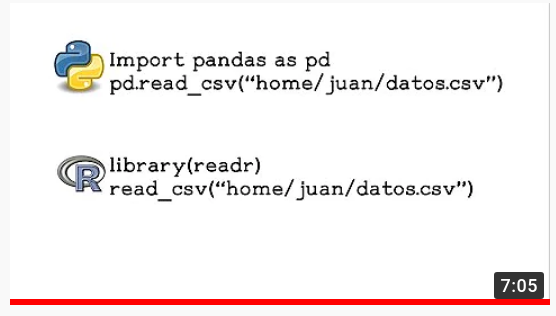
\includegraphics[width=.65\textwidth]{entendiendo.png}
\end{figure}
\centering
\textcolor{blue}{\url{https://youtu.be/Us0YyJtZRKE}}
\end{frame}


\section{Visualización de Datos}
\begin{frame}
\begin{center}
\Huge
\textcolor{azulcesaclaro}{2\\
--------------------------------\\
Visualización de Datos \\
(Primeras Sintaxis)}
\end{center}
\end{frame}

\begin{frame}
Con base en lo estudiado hasta este momento, usted debe generar un jupyter Notebook en el que se evidencie los siguientes elementos:\\
\vspace{0.5cm}
\begin{itemize}
\item Una sintaxis en donde usted es capaz de abrir el archivo newdata.csv explicado en el video anterior.
\vspace{0.3cm}
\item Una sintaxis en la que usted es capaz de aplicar alguna técnica sencilla de visualización de datos univariables (e.g., un histograma, un gráfico de torta, un gráfico de barras).
\vspace{0.3cm}
\item Una sintaxis en la que usted es capaz de aplicar alguna técnica sencilla de visualización de datos bivariables (e.g., scatterplot).
\end{itemize}

\end{frame}

\section*{REFERENCIAS}
\begin{frame}[allowframebreaks]{Referencias}
\tiny{ 
\bibliographystyle{apacite}
\bibliography{REFS.bib}
} 
\end{frame}

\setbeamertemplate{background}{\tikz[overlay,remember picture]\node[opacity=1]at (current page.center){
\includegraphics[width=18cm]{ulam.png}};}
\pgfdeclareimage[height=0cm,width=0cm]{}{}
 \logo{\pgfuseimage{}}
\beamertemplatenavigationsymbolsempty
\begin{frame}
\end{frame}
\end{document}